% q0028.tex — The "Beverage" Curve
\question{
  id        = {0028},
  title     = {The ``Beverage'' Curve},
  source    = {OBECON},
  year      = {2026},
  round     = {Seletiva IEO -- Phase B},
  language  = {English},
  topic     = {Macro},
  subtopic  = {Labor Markets / Beveridge Curve},
  type      = {dissertative},
  statement = {%
    Consider the following chart regarding the labor market in the United
    States from 2000 to 2025.

    \begin{center}
    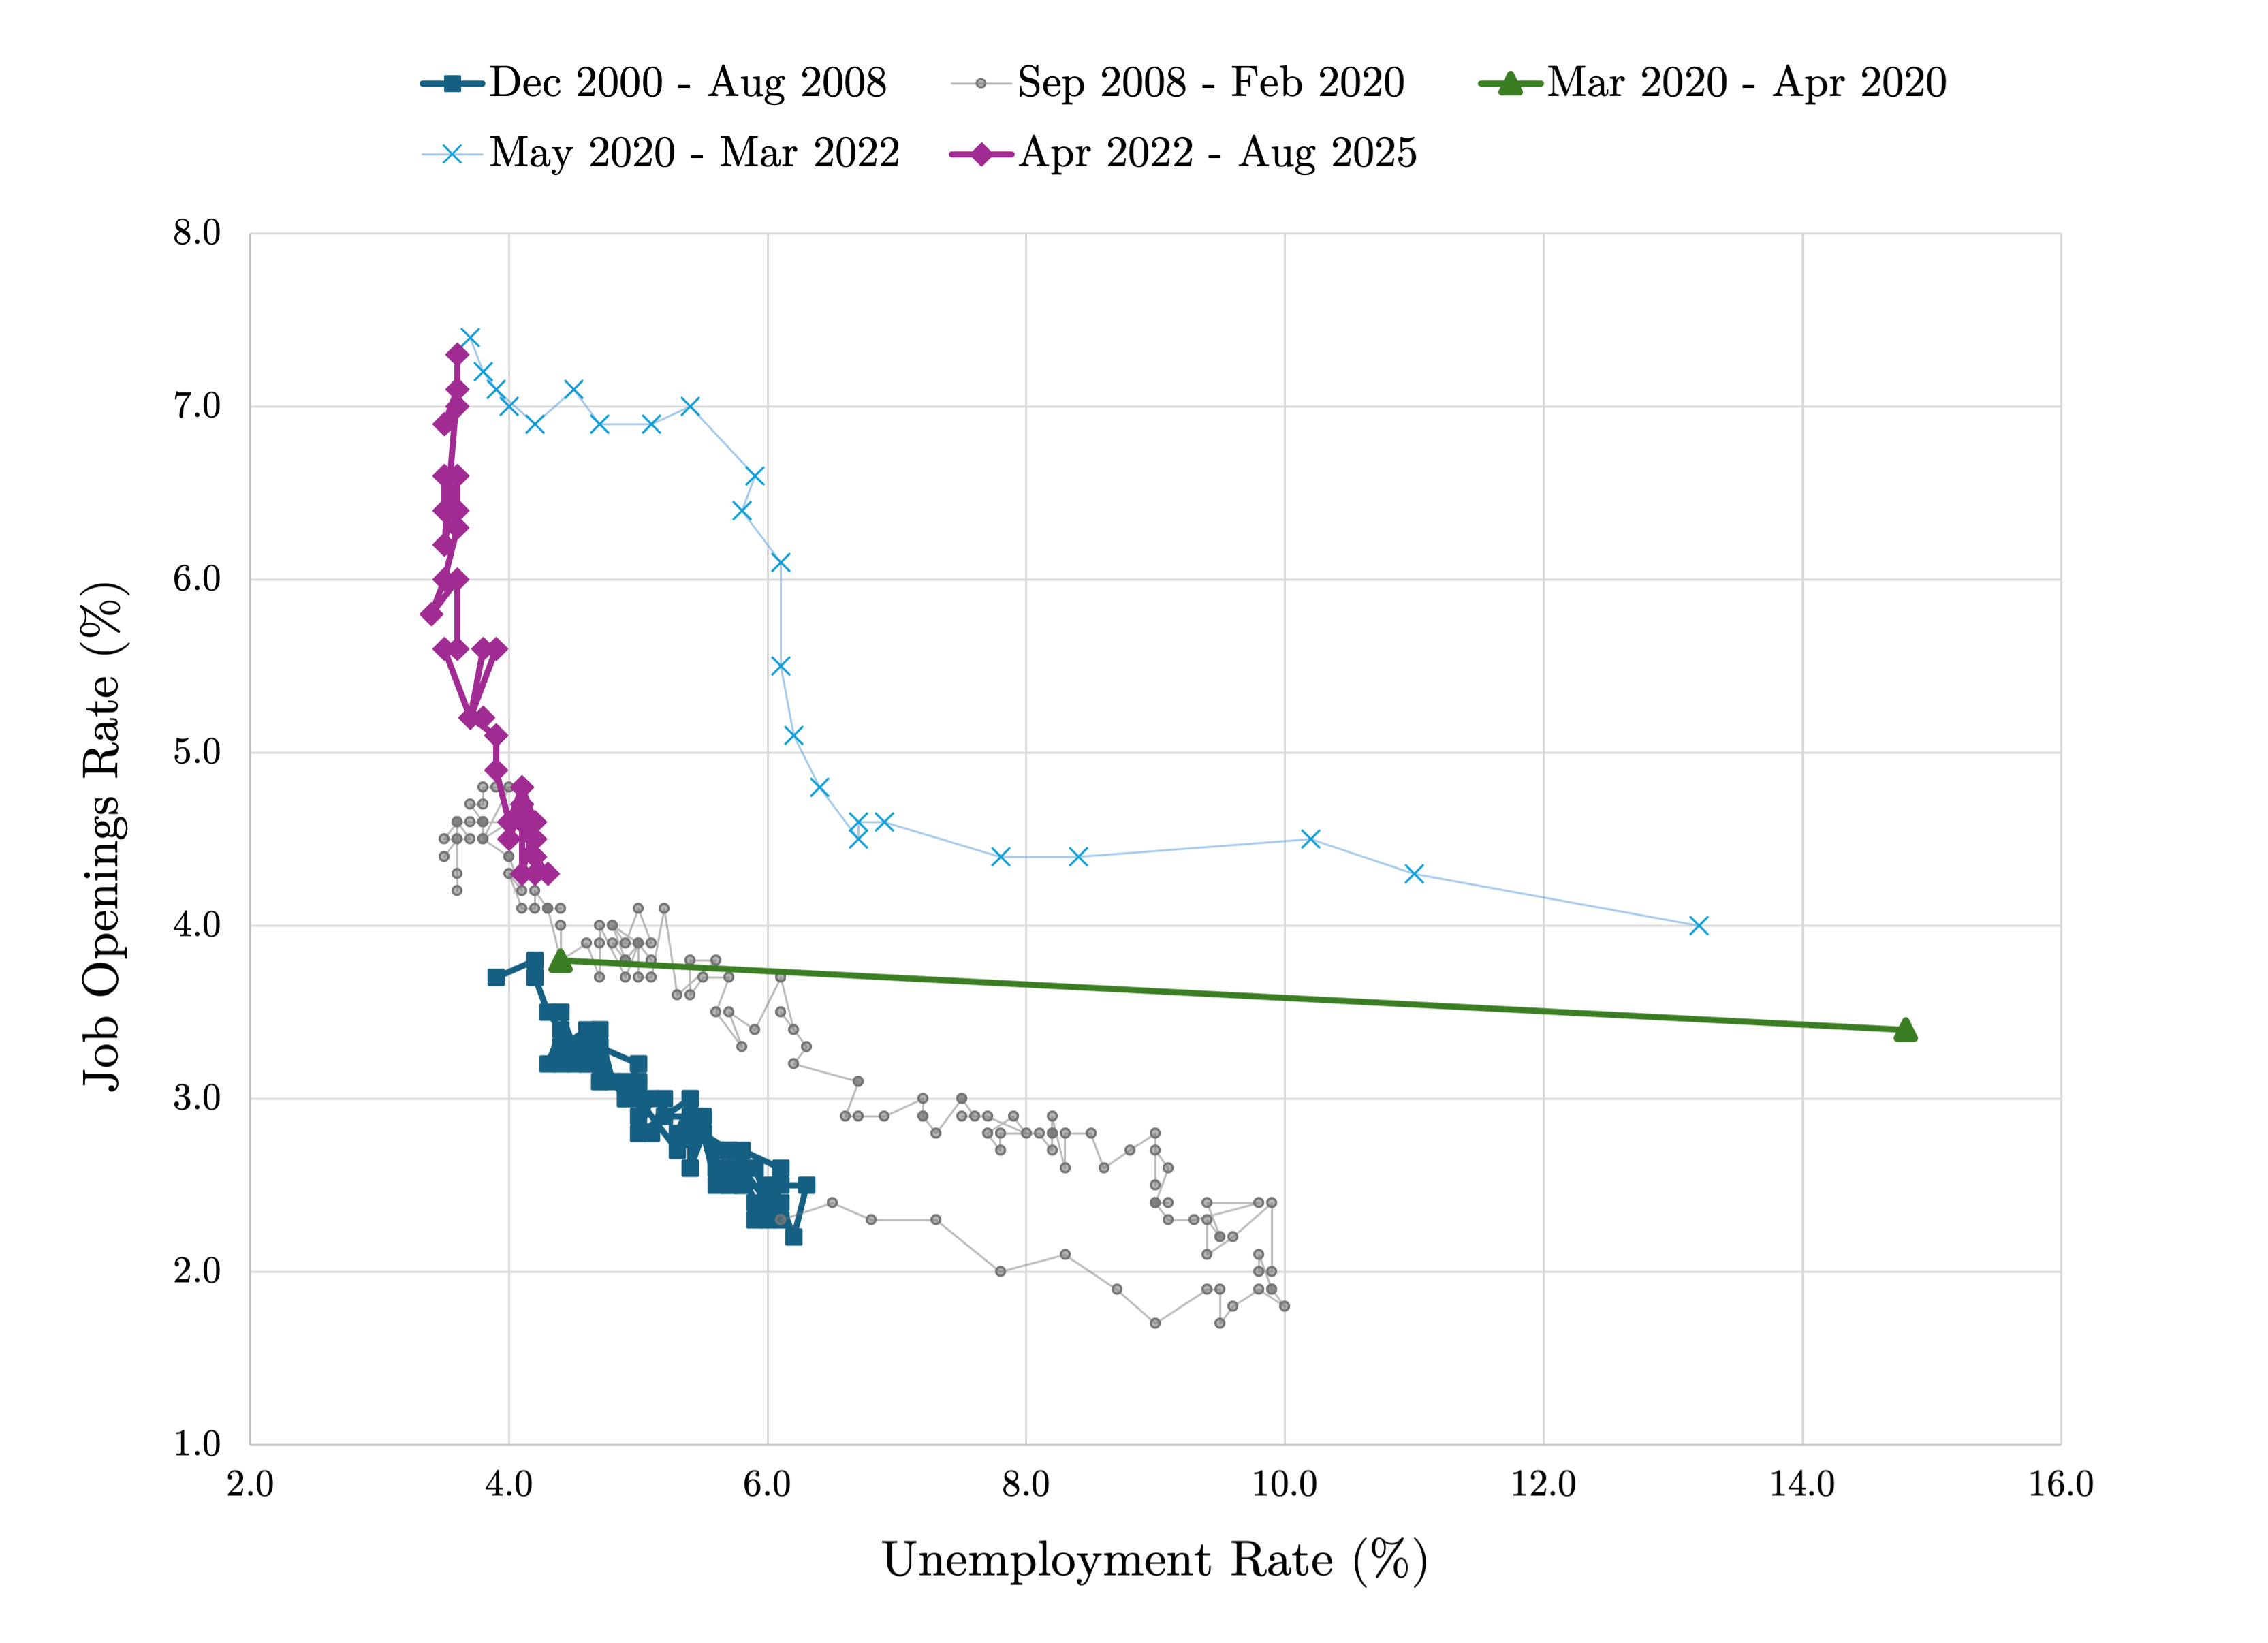
\includegraphics[width=0.85\textwidth]{../images/q0028_fig1.png}
    \end{center}

    \begin{enumerate}[(a)]
      \item (20 points) What is the relationship between unemployment and the
            job openings (vacancy) rate? Explain why this relationship exists.

      \item (20 points) As you can see, the green triangle line has only two
            dots, one in March 2020 and another in April 2020. Which dot do
            you think corresponds to March and which to April? What could
            explain such a sharp difference over this short period?

      \item (20 points) Let market tightness be defined as the ratio between
            vacancies ($v$) and unemployment ($u$), i.e.\ $\theta = v/u$.
            Based on the chart, how does market tightness in the period from
            April 2022 to August 2025 (purple rhombus line) compare to that
            from December 2000 to August 2008 (blue square line)?

      \item (20 points) What is the expected behavior of market tightness
            during a recession? And during an economic boom?

      \item (20 points) What relationship do you expect between market
            tightness and wage growth?
    \end{enumerate}
  },
  choices   = {},
  answer    = {},
  solution  = {%
    \textbf{(a)} There is a negative relationship between the unemployment
    rate and the vacancy rate. When the economy is doing well, businesses
    create more job openings to meet increased demand, lowering unemployment.
    Conversely, during downturns, businesses reduce hiring, raising
    unemployment. This downward-sloping locus is the \emph{Beveridge Curve}.

    \textbf{(b)} The dot to the left corresponds to March~2020, when
    unemployment was still low. The dot to the right (higher unemployment,
    lower vacancies) corresponds to April~2020, when COVID-19 lockdowns
    caused a sudden surge in unemployment and collapse in hiring.

    \textbf{(c)} From December~2000 to August~2008 market tightness was
    moderate and relatively stable. From April~2022 to August~2025 tightness
    increased significantly, with vacancies far exceeding unemployment,
    indicating an exceptionally tight labour market driven by strong
    post-pandemic demand.

    \textbf{(d)} During a recession, market tightness falls as unemployment
    rises and vacancies fall. During a boom, it rises as unemployment falls
    and vacancies increase.

    \textbf{(e)} There is typically a positive relationship between market
    tightness and wage growth. When $\theta$ is high, employers compete
    intensely for scarce workers and bid up wages. When $\theta$ is low,
    excess labour supply reduces wage pressure.
  },
}
